\chapter{IBM BigFix on SaaS, l'implementazione del prototipo}
L'attenta progettazione giudata dall'architect che abbiamo visto nel capitolo precedente è servita da base per la vera ralizzazione del prototipo che rappresenta l'aspetto implementativo del progetto BigFix SaaS. Ma queste due fasi del lavoro che stiamo presetando non sono l'una successiva l'altra. Infatti è bene rimarcare che, sguendo un approccio agile, iterativo e incrementale, l'intero disegno del progetto si è ottenuto solamente a fronte di una continua esplorazione dei requisiti che si è protratta durante tutta la fase implementativa. Il metronomo dello sviluppo sono state infatti le sprint demo, le quali vedevano la partecipazione anche di altri stackeholders interni all'azienda, oltre che al team stesso. Da questi confronti sono risultati continui feedback che hanno contribuito a portare il lavoro nel suo stato attuale.

\section{Container e microservizi di BigFix}
Per la necessità di continui feedback già dalla prima fase del progetto si è scelto di adottare, per i primi sprint, una soluzione intermedia per quanto riguarda la scomposizione del prodotto nei container. Si deciso infatti di fare in modo che, all'inizio, ogni container ospitasse un realay o un server di uno dei clienti forniti dal SaaS, e non un microservizio vero e proprio del prodotto. Questa scelta è avvenuta dopo un analisi dei requisiti. Scomporre BigFix in microservizi è un'operazione che richiede molte ore uomo di lavoro e affrontarla all'inizio del progetto non avrebbe consentito ti testare nelle primissime fasi le tecnologie che si erano individuate per il deployment. Avendo presto a disposizione gli ambienti cliente con relay e server, si sono subito testati scenari tipici del prodotto on premises nelle nuove tecnologie SaaS adottate.

\section{Gli ambienti di sviluppo }
La realizzazione di un progetto aziendale richiede più ambienti nei quali, sequenzialmente, viene testato il prodotto prima di metterlo sul mercato. L'ambiente ufficiale, quello di produzione, deve garantire tutti i parametri qualitativi di cui abbiamo parlato precedentemente. Per questo motivo è lì che si concentrano i maggiori investimenti a livello hardware per garantire alte prestazioni al servizio. Al tempo stesso però occorre avere a disposizione un "laboratorio" in cui sviluppare e testare il software, in cui implementare le nuove features quando il prodotto sarà già sul mercato, un ambiente nel quale le modifiche che si compiono al codice non impattino in nessun modo il servizio offerto ai clienti. Per questo motivo il primo contesto in cui si è andato a lavorare è l'ambiente di sviluppo. Un ambiente chiuso all'esterno dell'azienda, ma che al tempo stesso simulasse nella maniera più fedele possibile l'ambiente di produzione. A questi due si aggiunge un'ambiente intermedio di pre production, nel quale vengono svolti tutti i test qualitativi per verificare che il prodotto sia conforme ai parametri non funzionali stabiliti. 
\begin{figure}[h!]
	\centering
	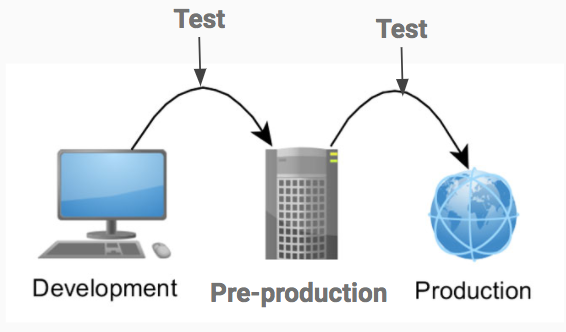
\includegraphics[width=0.7\textwidth,keepaspectratio=true]{capitoli/imgs/ambientisviluppo.png}
	\caption{Ambienti di BigFix SaaS}
\end{figure}

\section{Costruzione dell'ambiente e installazione di Docker e Kubernetes}
Vediamo una schematizzazione dell'ambiente di sviluppo nella figura 7.2. Kubernetes è il tool che muove le danze avendo proprio la funzione di orchestratore dei container. L'architettura di Kubernetes richiede che ci sia un nodo master che coordina i nodi denominati kube-node, che possono rappresentare macchine diverse. Su tutti i kube-node è installato anche docker, in quanto ci permetterà di ospitare su di essi i container. Questi vengono deployati su tutti i nodi a disposizione seguendo l'algoritmo di scheduling round-robin in modo da gestire al meglio le risorse di calcolo. 
\paragraph{}
Il Kubernetes master si interfaccia, come posiamo vedere, anche con altre due macchine presenti nella rete: La macchina DB2 e la macchina NFS. Andiamo a vedere di cosa si tratta.
\paragraph{DB2}
E' la macchina che ospita una replica del database. Spiegheremo in seguito come, nel processo di onboarding di un nuovo cliente, vengono dinamicamente allocate le risorse del database al nuovo utente.
\paragraph{NFS}
scrivere
\begin{figure}[h!]
	\centering
	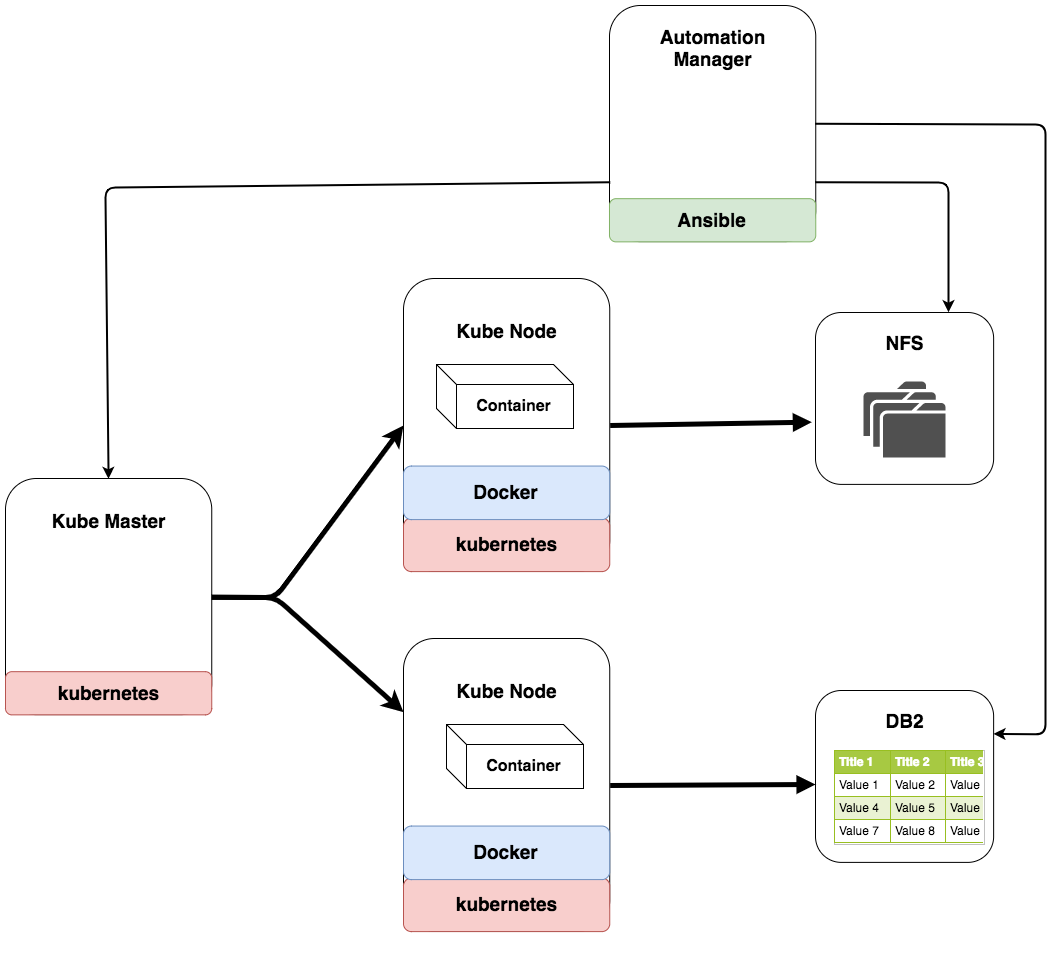
\includegraphics[width=0.5\textwidth,keepaspectratio=true]{capitoli/imgs/EnvironmentsComponentDiagram.png}
	\caption{L'ambiente di sviluppo di BigFix SaaS}
\end{figure}


\section{Re-working degli installer del server e del relay di BigFix}

\section{Generazione delle immagini Docker}
docker centos 7 
relay
server
cartelle di bigfix
install.sh
start.sh

\section{Docker containers, Pods e services}

\section{NFS vs Storage del container}

\section{Il database DB2 e il driver ODBC nei container}

\section{Relay scaling}

\section{Automazione del Deployment}
\subsection{Releases vs DevOps vs Continuous Delivery}
\subsection{Bash Scripting}
Nel progetto si è fatto largo uso del linguaggio Bash. Dovendo interagire con sistemi UNIX esso è stato spesso inserito in processi di automazione presenti nel 
\paragraph{Utilizzo degli script Bash nel progetto}
\subsection{Jenkins}
\subsection{UrbanCode}
\subsection{Ansible}

\section{Scenario di onboarding di un nuovo cliente}

\section{Scenario di upgrade del servizio}

\section{Automazione del Testing}
\subsection{Functional Test}
\subsubsection{JUnit}
\subsubsection{JUTAA}
\subsection{Security Test}
\subsubsection{AppScan}
\subsubsection{Image Compliance}
\subsection{Performance Test}
\subsection{Penetration Test}
\subsection{Rielaborazione degli output del testing}

\section{Scenario di testing}

\section{Il passaggio all'ambiente di produzione}
kubernetes -> ip pubblico, dns

